\documentclass[a4paper]{article}
\usepackage[a4paper,margin=0mm]{geometry}
\usepackage{fontspec}
\usepackage{unicode-math}
\usepackage{tikz}
\usepackage[table]{xcolor}
\usepackage[absolute]{textpos}
\usepackage{array}

\setmainfont{Libertinus Serif}
\setsansfont{Libertinus Sans}
\setmathfont{Libertinus Math}

\definecolor{accent}{HTML}{F46530}
\definecolor{badge}{HTML}{FFBDA5}
\definecolor{ink}{HTML}{2A2E30}

\setlength{\TPHorizModule}{1mm}
\setlength{\TPVertModule}{1mm}
\setlength{\parindent}{0pt}
\pagestyle{empty}

\newcommand{\pagefooter}[1]{%
\begin{textblock*}{194mm}(8mm,286.41mm)
  
\begin{tikzpicture}
    \fill[accent] (0,0) rectangle (194mm,0.6mm);
  \end{tikzpicture}
\end{textblock*}
\begin{textblock*}{63.59mm}(8mm,288.27mm)
  {\sffamily\bfseries\color{accent}\fontsize{13}{16}\selectfont SAT 1200+}
\end{textblock*}
\begin{textblock*}{10mm}(188mm,288.27mm)
  \centering{\sffamily\color{accent}\fontsize{14}{16}\selectfont #1}
\end{textblock*}
}

% ---- QR placeholder square + caption below ----
\newcommand{\qrbox}[1]{%
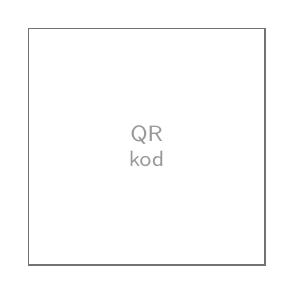
\begin{tikzpicture}
\draw[black!55,line width=0.6pt] (0,0) rectangle (30mm,30mm);
\node[black!40,font=\sffamily\fontsize{8}{9}\selectfont,align=center] at (15mm,15mm) {QR\\kod};
\end{tikzpicture}\\[1.5mm]
{\sffamily\bfseries\fontsize{9}{11}\selectfont\color{ink} #1}\\[1.5mm]
{\sffamily\fontsize{8.5}{11}\selectfont\color{black!45} @\makebox[20mm]{\dotfill}}%
}

\newcommand{\frontheader}[1]{%
\begin{textblock*}{194mm}(16mm,16mm)
\begin{tikzpicture}
\node[font=\sffamily\bfseries\fontsize{15}{16}\selectfont,text=ink,anchor=west] at (0,0) {#1};
\end{tikzpicture}
\end{textblock*}
\begin{textblock*}{194mm}(16mm,22.5mm)

\begin{tikzpicture}
\fill[accent] (0,0) rectangle (194mm,0.5mm);
\end{tikzpicture}
\end{textblock*}
}

\begin{document}

% ================= PAGE i: TITLE PAGE =================
\pagefooter{i}
\mbox{}%

\begin{textblock*}{160mm}(20mm,40mm)
{\sffamily\bfseries\fontsize{10}{12}\selectfont\color{ink} AVAZBEKOV SALOHIDDIN AZAMJON O'G'LI}
\end{textblock*}

\begin{textblock*}{3mm}(20mm,60mm)

\begin{tikzpicture}
\fill[accent] (0,0) rectangle (3mm,-110mm);
\end{tikzpicture}
\end{textblock*}

\begin{textblock*}{165mm}(32mm,58mm)
{\sffamily\bfseries\fontsize{48}{48}\selectfont\color{ink} SAT\\[2mm]1200+}
\end{textblock*}

\begin{textblock*}{150mm}(32mm,145mm)
{\sffamily\bfseries\fontsize{14}{18}\selectfont\color{accent} 1-KITOB \textperiodcentered\ ASOSLAR}
\end{textblock*}

\begin{textblock*}{150mm}(32mm,158mm)
{\sffamily\fontsize{11}{15}\selectfont\color{ink} O'zbekiston davlat universitetlari uchun tayyorlov}
\end{textblock*}

\begin{textblock*}{150mm}(20mm,255mm)
{\sffamily\fontsize{9}{13}\selectfont\color{black!55} Qisqa muddat ichida SAT uchun kerakli matematika\\va ingliz tili bilimlari}
\end{textblock*}

\newpage

% ================= PAGE ii: COPYRIGHT / LEGAL =================
\frontheader{Mualliflik huquqi}
\pagefooter{ii}
\mbox{}%

\begin{textblock*}{170mm}(20mm,34mm)
{\fontsize{10.5}{16}\selectfont\color{ink}

\textbf{\copyright\ 2026 Avazbekov Salohiddin Azamjon o'g'li. Barcha huquqlar himoyalangan.}

\vspace{4mm}
Ushbu kitobning biron qismini muallifning yozma ruxsatisiz ko'paytirish, qayta chop etish yoki sotish qat'iyan taqiqlanadi. Kitobni elektron, fotonusxa, skanerlash yoki boshqa har qanday usulda nusxalash mualliflik huquqini buzish hisoblanadi va qonun bo'yicha javobgarlikka olib keladi.

\vspace{4mm}
Birinchi nashr --- 2026, Chartak, Namangan viloyati, O'zbekiston.

\vspace{2mm}
Chop etildi: Chartak ZiyoFoto Studio.

\vspace{6mm}
{\fontsize{9}{13}\selectfont\itshape SAT\textregistered\ is a registered trademark of the College Board, which was not involved in the production of, and does not endorse, this product.}

\vspace{8mm}
\begin{tabular}{@{}p{14mm}p{140mm}@{}}
Muallif: & Avazbekov Salohiddin Azamjon o'g'li \\[2mm]
Telegram: & @tripplezet \\[2mm]
Email: & avazbekovsalohiddin19@gmail.com \\[2mm]
Tel: & +998 94 206 00 19 \\
\end{tabular}
}
\end{textblock*}

\newpage

% ================= PAGE iii: ABOUT THE BOOK =================
\frontheader{Kitob haqida}
\pagefooter{iii}
\mbox{}%

\begin{textblock*}{170mm}(20mm,34mm)
{\fontsize{11}{16}\selectfont\color{ink}

\textbf{SAT 1200+} --- Digital SAT imtihonining matematika bo'limiga tayyorlanish uchun yozilgan uch kitoblik seriya. Har bir kitob talabani asta-sekin yuqori ball tomon olib boradi: \textbf{1-kitob} asosiy matematik fundamentni mustahkamlaydi, \textbf{2-kitob} SATning asosiy mavzularini (algebra, funksiyalar, statistika, geometriya) to'liq ingliz tilida yoritadi, \textbf{3-kitob} esa yuqori ballga erishish uchun murakkab masalalar va tezlik strategiyalarini o'rgatadi.

\vspace{4mm}
Ushbu kitob zamonaviy, ma'lumotlarga asoslangan metodika asosida tuzilgan: har bir mavzu College Board'ning rasmiy savollar bazasi tahlili, O'zbekiston maktab dasturi bilan moslik va xalqaro ta'lim tizimlaridagi eng yaxshi amaliyotlarni hisobga olgan holda tanlangan.

\vspace{4mm}
\textbf{Har bir darsning tuzilishi:}

\vspace{2mm}
\begin{tabular}{@{}p{10mm}p{150mm}@{}}
1. & \textbf{Qoida/Formula sahifasi} --- mavzuning eng muhim qoidalari bitta sahifada, aniq misollar bilan. \\[3mm]
2. & \textbf{Tushuncha (Concept)} --- har bir mavzu ta'rif, yechilgan misol va mashq bilan tushuntiriladi. \\[3mm]
3. & \textbf{Lug'at (Vocabulary)} --- SAT savollarida uchraydigan ingliz tilidagi atamalar o'zbekcha tarjimasi bilan. \\[3mm]
4. & \textbf{Mashqlar (Problems)} --- bosqichma-bosqich qiyinlashib boruvchi mashqlar to'plami. \\
\end{tabular}

\vspace{6mm}
Kitob oxirida esa barcha 9 ta darsda uchragan so'zlarni o'z ichiga olgan \textbf{to'liq lug'at (complete glossary)} berilgan --- bu 2-kitobga o'tishda talaba allaqachon tanish bo'lgan ingliz tilidagi SAT lug'ati bilan qurollangan bo'ladi.

}
\end{textblock*}

\begin{textblock*}{170mm}(20mm,218mm)
{\sffamily\bfseries\fontsize{11}{14}\selectfont\color{ink} Bizni kuzating}
\end{textblock*}

\begin{textblock*}{170mm}(20mm,225mm)

\begin{tikzpicture}
\fill[accent] (0,0) rectangle (170mm,0.4mm);
\end{tikzpicture}
\end{textblock*}

\begin{textblock*}{170mm}(20mm,233mm)
\centering
\begin{minipage}[t]{30mm}\centering\qrbox{Telegram}\end{minipage}%
\hspace{20mm}%
\begin{minipage}[t]{30mm}\centering\qrbox{YouTube}\end{minipage}%
\hspace{20mm}%
\begin{minipage}[t]{30mm}\centering\qrbox{Instagram}\end{minipage}
\end{textblock*}

\end{document}
